\section{Auction-SC Algorithms}
\label{sec:onlinealgo}

Without the global knowledge about future tasks and workers, in practice, it is not feasible for an SC-Server to produce optimal assignments. Furthermore, even for a small number of tasks and workers, finding the optimal assignment is challenging due to the high complexity of the clairvoyant algorithm. In this section, we propose Auction-SC, a scalable auction-based framework that splits the assignment and scheduling responsibilities between the SC-Server and workers. We present several bidding techniques that the SC-Server can utilize to select a worker to assign to each task.

Auction methods have been effectively used for assignment problems in dynamic multi-agent environments \cite{Mehta05,Lagoudakis04}. Auction-SC considers the workers as bidders and tasks as goods. Upon arrival of each task, it performs one round of bidding. During each round of bidding, all workers bid on the task. Depending on the bidding rule, the worker with the overall highest/lowest bid wins and is assigned to that particular task. Upon assignment of a new task, each worker updates its schedule based on the task(s) that it has been assigned to and moves along its path.

The main advantage of Auction-SC is its simplicity and the fact that it allows for a decentralized implementation. In each round, each worker computes its bid locally and in parallel with the other workers and reports the bid to the SC-Server. Each worker only needs to know its own location, the location of the new task but not the location of any other worker. The SC-Server, which plays the role of a central auctioneer, chooses the winning worker and assigns the task. It is worth noting the low cost of communication in Auction-SC; each worker submits only one number to the SC-Server in each round of bidding. In addition, workers do not have to share their location with any other entity (including the SC-Server) which preserves their privacy to some level \footnote{Later, we see the bidding technique may reveal a coarse location of the user}.

\begin{algorithm}
\caption{OnlineTASC($W, t$)}
\label{algo:OnlineTASC}
\begin{algorithmic}[1]
\REQUIRE $W$ is the set of currently available workers and $t$ is a task the has just released
\ENSURE Either $w \in W$ as the worker task $t$ should be assigned to or \emph{null} if no worker is selected
\STATE $w_{selected} = $ \emph{null}
\STATE $Bids = \emptyset$
\FOR{$w \in W$}
	\STATE $bid = w$.ComputeBid$(t)$
	\STATE $Bids \leftarrow \left\langle w, bid \right\rangle$
\ENDFOR
\STATE $w_{selected} = $ SelectBestBid$(Bids)$
\RETURN $w_{selected}$
\end{algorithmic}
\end{algorithm}

\cref{algo:OnlineTASC} outlines the process of assigning an incoming task $t$. Notice that all the iterations of the \textbf{for} loop in \cref{algo:OnlineTASC} (lines 3-6) runs in parallel. The \emph{ComputeBid()} method (line 4) that each worker executes depends on the implemented bidding rule. Similarly, the \emph{SelectBestBid()} method (line 7) returns the worker with either the highest or lowest bid. In case of a tie, the \emph{SelectBestBid()} method, randomly selects one worker among the ones with optimum bid.

In the remainder of this section, we discuss different bidding rules that can be leveraged to maximize the quality of the assignment. First, we introduce four bidding rules that do not consider scheduling. Neither one of these rules consider both spatial and temporal characteristics of SC at the same time, hence we call them non-SC rules. When a non-SC rule is in effect, once a task is assigned, only the selected worker needs to perform scheduling. In certain cases the worker may not be able to schedule all its assigned tasks. subsequently we introduce two rules that require scheduling during the bidding phase (SC rules).

Before submitting a bid, each worker performs an eligibility check and only eligible workers proceed with bidding. For non-SC rules, each worker examines if regardless of its current schedule, it can reach the task's location before either it leaves the system or the task's deadline. The four non-SC rules we propose are based on \emph{Online Bipartite Matching} \cite{Karp90}, \emph{Spatial Matching} \cite{Wong07} and \emph{Online Scheduling} \cite{Lee13} problems.

\vspace{0.1in}
\noindent\textbf{Random (Rnd)}:
As a baseline approach, we consider a rule where every eligible worker submits a bid of value 1. The SC-Server selects the winner randomly from the set of eligible workers.

\vspace{0.1in}
\noindent\textbf{Ranking (Rnk)}:
Based on the ideas in online bipartite matching \cite{Karp90}, the workers are ranked from 1 to $n$ (the order of the workers does not change over time). Each eligible worker submits a bid of value 1 and the SC-Server selects the eligible worker with the lowest rank as the winner.

\vspace{0.1in}
\noindent\textbf{Nearest Neighbor (NN)}:
Similar to the \emph{Nearest Neighbor Priority Strategy} in \cite{Kazemi12}, for this bidding rule we give priority to the closest worker to the location of the task. To compute a bid, each worker needs to compute the distance between the location of the task and its own location. Once every worker has submitted its bid, the SC-Server chooses the worker with the minimum bid as the winner.

\vspace{0.1in}
\noindent\textbf{Most Free Time (MFT)}:
In this bidding rule, we give priority to workers that have more time before they leave the system. Since at each point of time, each worker has a schedule, we compute the worker's \emph{free time} as the time between when it finishes its current schedule and the time it leaves the system. Each worker submits a bid equal to its \emph{free time} and the SC-Server selects the worker with the highest bid as the winner.

\subsection{SC (Bidding) Rules }

To reduce the number of incomplete tasks inflicted by non-SC bidding rules, we propose the following two SC rules that enable simultaneous task assignment and scheduling. The main difference between SC and non-SC rules is that SC rules take scheduling and the dynamism of SC environments into consideration. For a worker to be \emph{eligible} when SC rules are in effect, there should exist a schedule that can fit the incoming task to the worker's current schedule. Similar to non-SC rules, only eligible workers are allowed to submit a bid. This guarantees the completion of all assigned tasks.\\

\noindent \textbf{Best Insertion (BI)}: 
Intuitively, if a worker travels less to complete a task it will likely have more time for performing other tasks. For this bidding rule, we give priority to workers that can better insert the current task into their schedules. Here we consider the \textit{additional} time each worker will need to complete the new task in addition to the incomplete tasks already assigned to it.

For this bidding rule each worker starts with finding the optimal schedule in case the task is assigned to it. For this the worker uses a branch and bound algorithm similar to \cref{algo:SearchBranch} to check all possible orders of its uncompleted tasks in addition to the new task. Running an exhaustive search for large number of tasks can be time consuming. However, in our experiments with both real world and synthetic data, we realized that the number of completed tasks for each worker always remains in a range where even the exhaustive search can be done in real-time. The reason is that as time passes and new tasks arrive, the worker completes other tasks and removes them from its schedule. In cases where computing the bid takes too long, we can replace this computation with an approximate algorithm (e.g., the Nearest Insertion algorithm \cite{Rosenkrantz74}).

In order to compute a bid, each worker finds the finish time of its current schedule $(f_1)$. The worker also finds the finish time of the optimal schedule in case the task is assigned to it ($f_2$). Subsequently, the worker's bid is $f_2 - f_1$. The SC-Server assigns the task to the worker with the lowest bid.\\

%\item \textbf{Best Distribution}

%The general idea behind this heuristic is to try to move workers to locations where there is a higher chance for future tasks to be located around. Ideally, we want the spatial distribution of the \textit{current} workers $(S_W)$. to be as close as possible to the \textit{overall} spatial distribution of the tasks $(S_T)$.\\
%One can argue that knowing $S_T$ contradicts the assumption that the SC server has no spatiotemporal knowledge about future tasks. However, even if the server knows $S_T$ doesn't mean it also knows the exact location where the task is going to be released. Even if we don't want the server to know $S_T$ as a priori, we can assume that the server starts with an empty distribution and keeps updating it as new tasks arrive. During each round of bidding, the server shares the most updated version of $S_T$ with workers.\\
%We show a spatial distribution using a grid and count the number of events in each cell. By normalizing the counts, we can come up with the probability of an event occurring in each cell.

\noindent \textbf{Best Distribution (BD)}: 
BI does not consider the spatial distribution of tasks. For example, it may be beneficial to assign a task located at a task-dense area to a worker with high remaining availability, even if it has to deviate from its current path significantly. The general idea behind this rule is to try to move workers to locations where there is a higher chance for future tasks to be located in. Ideally, we want the spatial distribution of the \textit{available} workers $(S_W)$ to be as close as possible to the \textit{overall} spatial distribution of the tasks $(S_T)$.

One can argue that knowing $S_T$ contradicts the assumption that the SC-Server has no spatiotemporal knowledge about future tasks. However, even if the SC-Server knows $S_T$, it does not mean it also knows the exact location where the tasks are going to be released at. However, we don't make the assumption that $S_T$ is known a priori. Instead, we assume that each worker starts with an empty distribution and keeps updating it as new tasks arrive. Also, earlier we mentioned in Auction-SC the workers don't have to share their exact location with the SC-Server. 

We show a spatial distribution using a grid and for each event occurring inside a cell, we add to the weight of that cell. To compute $S_T$, for every task we add a value of 1 to the cell the task resides in. As for $S_W$, we need to consider the \textit{availability} of the worker. For example, if the maximum number of tasks worker $w$ can perform is $n$, and it already has been assigned $m$ tasks, we say the availability of worker $w$ is $n-m$. In this case, when computing $S_W$, we add $n-m$ units to the cell covering $w$. For both $S_T$ and $S_W$, by normalizing the weights of the cells, we can compute the probability of an event occurring in each cell.

Having $S_W$ and $S_T$, we need a metric to determine how close these two distributions are. Several methods have been used to compute the similarity between two distributions. Among the more commonly used methods, we can name the Kullback-Leibler divergence \cite{Kullback51} and Jensen-Shannon divergence \cite{Lin91}. The problem with these methods is that they do not take the spatial attribute of the cells into consideration. For example, \cref{fig:sdist} shows the two spatial distribution for two tasks (red dots) and two workers (blue squares). Clearly, in \cref{fig:sdist2} the distribution of workers is more similar to $S_T$ compared to the distribution of workers in \cref{fig:sdist1}. However, if we consider the Jensen-Shannon divergence metric, then $JSD(S_T, S_{W_1})$ is going to be equal to $JSD(S_T, S_{W_2})$. The same happens if we consider the Kullback-Leibler divergence or any other measure that does not take into account the spatial relationship between the cells.

\begin{figure}[t]
    \centering
    \subfigure[Distribution 1]{
        \label{fig:sdist1}
        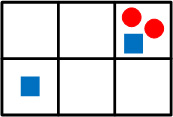
\includegraphics[scale=0.5]{figures/sDist1.jpg} }
    \subfigure[Distribution 2]{
        \label{fig:sdist2}
        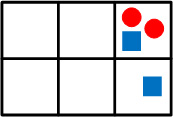
\includegraphics[scale=0.5]{figures/sDist2.jpg}
    }
    \caption{Two spatial distributions for tasks and workers}
    \label{fig:sdist}
\end{figure}

To account for spatial features of the distribution, in this paper, we use the \textit{Earth Mover's Distance} metric since it has the ability to incorporate the spatial aspect of the distributions when computing their similarity.

\begin{definition}[Earth Mover's Distance]
The Earth Mover's Distance (EMD) is a measure of distance between two probability distributions over a region $D$. If the distributions are interpreted as two different ways of piling up a certain amount of dirt over region $D$, the EMD is the minimum cost of turning one pile into the other; where the cost is assumed to be the amount of dirt moved, times the distance by which it is moved \cite{Rubner98}.
\end{definition}

For each grid cell $i$, we call cell $i$ a supplier iff $P_A(i) > P_B(i)$ and a consumer iff $P_A(i) < P_B(i)$. If $P_A(i) = P_B(i)$, cell $i$ is neither a supplier nor a consumer. For each supplier $i$, we say $a_i = P_A(i) - P_B(i)$ is the total supply of $i$. Also, the total demand for consumer $j$ is shown as $b_j = P_B(j) - P_A(j)$. Now we can model the problem as a bipartite network flow problem where on one side we have the suppliers and on the other side we have consumer nodes (\cref{fig:MinFlow}). The weight of each edge $c_{ij}$ between supplier $i$ and consumer $j$, is the cost of moving one unit of mass from $i$ to $j$.  Consequently, finding EMD reduces to finding the \textit{Minimum Cost Flow} for this bipartite graph. The Minimum Cost Flow problem can be formalized as the following linear programming problem:

\begin{figure}[t]
  \centering
  \label{fig:MinFlow}
  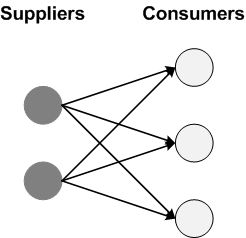
\includegraphics[scale=0.4]{figures/MinFlow.png}
  \caption{Example of MinFlow Problem}
\end{figure}

\setcounter{equation}{0}
\begin{alignat}{2}
\mathbf{minimize}&\mathrlap{\sum_{i \in \mathcal{I}} \sum_{j \in \mathcal{J}} c_{ij}.f_{ij}} \notag\\
\mathbf{subject\ to:}&\phantom{{a}={a}} f_{ij} && \geq 0 \ \quad\quad i \in \mathcal{I}, j \in \mathcal{J}\\
&\phantom{{a}}\sum_{i \in \mathcal{I}} f_{ij} &&= b_j \quad\quad j \in \mathcal{J}\\
&\phantom{{a}}\sum_{j \in \mathcal{J}} f_{ij} &&\leq a_i \quad\quad i \in \mathcal{I}
\end{alignat}

More generally, for any graph $G = (V, E)$ we can assign an integer $b(i)$ to each node in the graph, which indicates the supply (or demand) of the node if $b(i) > 0$ (or $b(i) < 0$) . Then we can rewrite the linear programming problem as: 

\setcounter{equation}{0}
\begin{alignat}{2}
\mathbf{minimize}&\mathrlap{\sum_{(i,j) \in \mathcal{E}} c_{ij}.f_{ij}} \notag\\
\mathbf{subject\ to:}&\phantom{{a}={a}{a}={a}{a}={a}{a}} f_{ij} && \geq 0 \ \quad\quad (i,j) \in \mathcal{E}\\
&\sum_{j:(j,i) \in \mathcal{E}} f_{ij} - \sum_{j:(i,j) \in \mathcal{E}} f_{ij} &&= b(i) \quad\quad i \in \mathcal{V}
\end{alignat}

\noindent We can solve this LP problem using the simplex method \cite{Dantzig90}.

In this bidding rule, each worker needs to know $S_W$ in order to be able to compute the EMD for $S_W$ and $S_T$. We assume the SC-Server keeps track of the current $S_W$ and shares it with the workers. First, each worker has to fit the incoming task into its current schedule. If the worker is able to find a new schedule, it can generate a local modification of $S_W$, i.e., $S_{W}'$, with its final location and remaining availability at the end of the updated schedule. Subsequently, the worker computes the EMD between $S_{W}'$ and $S_T$ and submits the value as its own bid. The SC-Server selects the worker with the lowest bid as the winner. In our implementation, we simplex method \cite{Dantzig90} to efficiently solve the LP problem for EMD. Our empirical evaluation shows the average computation time per task is within 3 milliseconds. 

%We use a variation of the algorithm proposed in \cite{Edmonds72}. The solution in \cite{Edmonds72} is based on solving the dual of the linear programming problem:

%\setcounter{equation}{0}
%\begin{alignat}{2}
%\mathbf{maximize}&\quad\mathrlap{\sum_{i \in \mathcal{V}} b(i).\pi(i)} \notag\\
%\mathbf{subject\ to:}&\quad\pi(i) - \pi(j) \leq c_{ij} \quad\quad (i,j) \in \mathcal{E}
%\end{alignat}

%\begin{algorithm}[t]
%\caption{MinFlow($V, E, b$)}
%\label{algo:MinFlow}
%\begin{algorithmic}[1]
%\REQUIRE $V$ is the set of nodes, $E$ the set of edges and $b$ the supply/demand of each node
%\ENSURE $f$ as the amount of flow on each edge
%\STATE for $i \in V$ set $f_i = 0, \pi_i =0$ and $e_i = b_i$
%\STATE $U = \max_{i \in V} \left\lbrace\vert b_i\vert \right\rbrace$
%\STATE $\delta = 2^{ \lceil \log U \rceil }$
%\WHILE {$\delta \geq 1$}
%   \STATE $S_{\delta} = \left\lbrace i : e_i \geq \delta \right\rbrace$
%   \STATE $C_{\delta} = \left\lbrace i : e_i \leq -\delta \right\rbrace$
%   \WHILE{$S_{\delta} \neq \emptyset$ and $C_{\delta} \neq \emptyset$}
%     \STATE choose some $s \in S_{\delta}$
%     \STATE compute shortest path distances $d_i$ from node $k$ to all other nodes
%     \STATE for $i \in V$ set $\pi_i = \pi_i - d_i$
%     \STATE choose $c \in C_{\delta}$ such that a path exists from $s$ to $c$
%     \STATE augment $\delta$ units of flow along the shortest path from $s$ to $c$
%     \STATE update $f, e, S_{\delta}$ and $C_{\delta}$
%   \ENDWHILE
%   \STATE $\delta = \frac{\delta}{2}$ 
%\ENDWHILE
%\RETURN $f$
%\end{algorithmic}
%\end{algorithm}

%\cref{algo:MinFlow} is based on the ideas proposed in \cite{Edmonds72}. In line 9, we use Dijkstra's algorithm to compute shortest paths from node $s$ to all other nodes. Instead of using the normal cost of each edge, $c_{ij}$, in computing the shortest paths, \cref{algo:MinFlow} uses a modified cost, $c_{ij}^{*} = c_{ij} - \pi_i + \pi_j$, as the cost of each edge in line 9. It is shown in \cite{Edmonds72} that \cref{algo:MinFlow} runs in polynomial time.